\chapter{Overview}
\label{chap:Overview}
\section{Motivation}
\label{sec:Motivation}
Neuronal models of reinforcement learning assume interactions of midbrain dopaminergic neurons and striatum to compute the differences between anticipated and received outcomes. The nature of this cross-areal interaction is however not fully understood. On this purpose we recorded dual site simultaneous electrophysiological in-vivo data from Ventral Striatum, including Pallidum, (VS) and Ventral Tegmental Area (VTA). On this data set we applied a cell assembly detection algorithm (\cite{RussoDurstewitz}).
The novel statistical approach presented treats the temporal scale and precision of coherent activity patterns as free parameters, to be determined from the data, thus, instead to make assumption, we deduced from data temporal scales and precision involved in assemblies pairs with units either from both regions or from only one of the two regions, shedding light on VS-VTA interaction temporal structure and VS-VTA directionality.
We can use the term directionality in our case because we use the algorithm at level of inter-regional pairs. It is important to recall that the cell-assembly algorithm returns lags between the units activation in assembly, thus using the algorithm at level of inter-regional pairs provides us the lag between two units activation, of those two units one is in VS and another in VTA, a lag in activation of such kind of pair, indicates which region is preceding the other in activation.
Our nomenclature was such that a positive lag means that VS is prior in activation, a negative lag, vice-versa, means that VTA is preceding the activation of VS.
Taking advantage of well defined neuron typologies classifications both in VS and VTA, we further investigated the specific cell-type composition of the assemblies exhibiting directionality. 
{\color{red}da finire}
%Using the bin size distribution
\section{State of the art}
\label{sec:StateArt}
 In recent decades Ventral Striatum and Ventral Tegmental area have been widely studied by scientists because of their prediction coding feature.
 To introduce the study on VS-VTA interaction an overview on the state of the art of the Ventral Striatum and Ventral Tegmental area knowledge is needed.
\section{Experiment and data set}
\label{chap:Dataset}
In this chapter I describe the task and the data collected in our lab.
The task presented is a go/no-go reversal odor discrimination task. Two odors were presented to the mouse, one rewarded (CS+) with reward probability 0.9, the second one unrewarded (CS-). Learning the task consisted in licking at least a defined number of times (two or three depending on the paradigm) during a specific interval, called lick window, when the rewarded odor (CS+) was presented (hit trials) and not licking when unrewarded odor (CS-) was presented (correct rejection trials). Whereas a bad performance consisted in not licking, or licking outside the lick window period, at CS+ presentation (miss trials), or licking at CS- presentation (false alarm trials). Once the performance criterion was reached, the contingencies were switched, in other words the rewarded odor became unrewarded and vice-versa. Once the performance criterion was reached in the reversal phase the extinction phase followed, in which neither one of the two odors was rewarded. The lick window was open for an interval ranging from 1500 $ms$ to 2000 $ms$ depending of different paradigms. after a delay from 500 $ms$ to 1500 $ms$. Only licks happening in the lick window interval were counted as valid to get the reward.
\begin{figure}
    \centering
    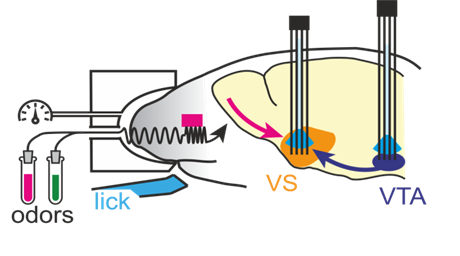
\includegraphics[scale=1]{figures/Experiment.png}
    \caption{Scheme of the experimental setup. Two odors in randomized sequences were presented, the mouse was head-fixed and, to get the reward, had to lick during the allowed licking period when the rewarded odor was presented. Electrodes were implanted in Ventral Striatum and Ventral Tegmental Area to record the neural activity. }
    \label{fig:experiment}
\end{figure}

\begin{figure}
    \centering
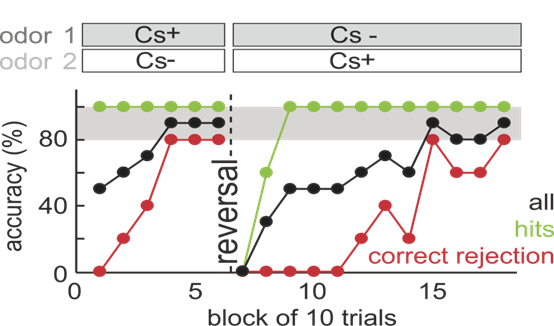
\includegraphics[scale=1]{figures/Performance.png}
\caption{Example of one animal's performance in original and reversal phase. In the shown paradigm the performance criterion to be reached to switch to the reversal phase was $79\%$, meaning that this level of accuracy had to be satisfied for hit trials and correct rejection trials. Black line indicates global performance including hit trials and correct rejection trials. Green line is the performance for the performance in hit trials and red lines is the performance in correct rejection trials.}
\label{fig:performance}
\end{figure}
\section{Cell assembly detection method}
\label{chap:AssemblyMethod}
\subsection{Introduction}
\subsection{Method}